\question{10.m2}{
    Bij een chikwadraattoets voor onafhankelijkheid moet worden gewerkt met de chikwadraatverdeling met $6$ vrijheidsgraden.
    Er moet worden getoetst met $\alpha=0,05$.
    De kritieke tabelwaarde is daarom $\ldots$
}
\begin{enumerate}[label=(\alph*)]
    \item $1,64$
    \item $14,45$
    \item $12,59$
    \item $9,49$
\end{enumerate}
\answer{
    Laat $X$ de toetsingsgrootheid zijn die chikwadraat verdeeld is met df$=6$ vrijheidsgraden.
    In dit geval is de kritieke waarde de waarde $x$ waarvoor geldt dat $P(X \ge x) = 0,05$.
    Deze kritieke waarde berekenen we met de solver optie als volgt:
    \begin{align*}
        y_1 &= \chi^2\text{cdf}(\text{lower}=x; \text{upper}=10^{10}; \text{df}=6) \\
        y_2 &= 0,05
    \end{align*}
    De numerieke solver geeft (afgerond op twee decimalen) $x \approx 12,59$.
    Het juiste antwoord is dus (c).

    \begin{center}
        \resizebox{0.9\textwidth}{!}{
            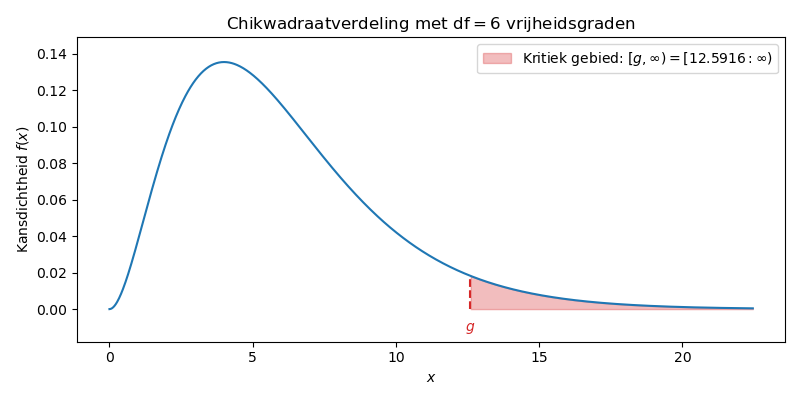
\includegraphics{opg_10.m2.png}
        }
    \end{center}
}
